\begin{figure*}[t]
  \centering
  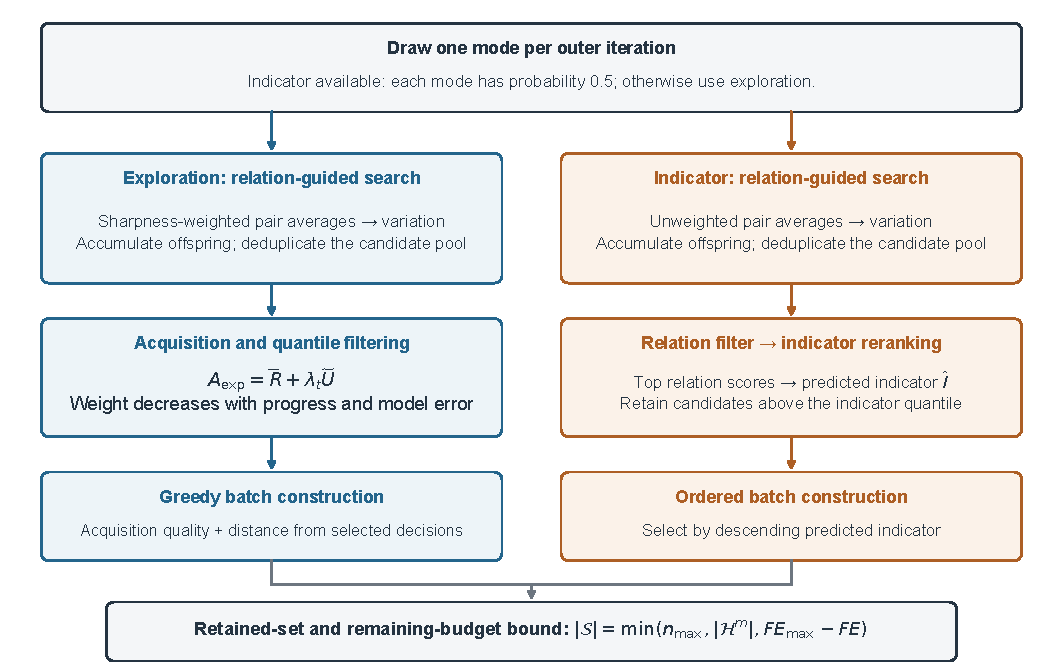
\includegraphics[width=0.98\textwidth]{figures/fig_candidate_selection.pdf}
  \caption{Dual-mode candidate selection. A mode is drawn before the inner
  search, so its relation aggregation also influences candidate generation.
  The two branches represent alternative executions under the same
  pool-construction rule. Exploration combines relation quality, prediction
  ambiguity and decision-space separation; indicator selection applies relation
  filtering followed by predicted-indicator reranking. Each retained set is
  completed to $n_{\min}$ when needed and when the pool permits, before the
  batch and remaining-budget bounds are applied. The empty-pool fallback is
  stated in Algorithm~\ref{alg:framework}.
  \label{fig:candidate-selection}}
\end{figure*}
